\chapter{Analysis and Results}\label{chap:results}
\begin{jointwork}
    Data analysis procedures and searches for Milky Way ALPs are adapted from Ref.\,\cite{Walter2025_CASPErLFthermal}, a publication by the author and collaborators.
    The analysis framework was developed using the data analysis pipelines of HAYSTAC\,\cite{Brubaker2017_HAYSTAC}, SHAFT\,\cite{Gramolin2021_Ferromagnetic}, and CASPEr-Electric\,\cite{aybas2021_SolidStateNMR} as references.
\end{jointwork}

This chapter first presents the data analysis pipeline, including data processing and candidate validation.
The data analysis pipeline is later applied to two proof-of-principle ALP searches using the CASPEr-Gradient-LF apparatus with a thermally polarized methanol sample.
The results, including the analysis of ALP candidates and the exclusion limits, are presented at the end of the respective sections.


\section{Data analysis}\label{sec:results:data_analysis}

% purpose of the data analysis
The data analysis of CASPEr-Gradient aims at identifying potential ALP signals in the frequency spectra obtained from the measurements and setting exclusion or sensitivity on the ALP coupling in the absence of a detection.


\subsection{Methodology}\label{sec:results:data_analysis:methodology}

% summary of the data analysis procedure
In general, the raw time-series data are first converted to the frequency domain using a Fourier transform, and then processed with filters to suppress noise.
The outliers in the filtered spectra, judged by a threshold determined from Monte Carlo (MC) simulations, are later evaluated for their consistency across repeated scans.
\textbf{Outliers} that survive the consistency checks are considered ALP \textbf{candidates}.
If no candidate is found in a frequency band, the analysis sets an exclusion limit on the ALP-nuclear spin gradient coupling in this band.

% more details about the general data analysis procedure
A more detailed description of the data-analysis procedure is given below and summarized in Figure~\ref{fig:casper_g_data_analysis_pipeline}.
The analysis consists of 4 main stages:
\begin{itemize}
    \item \textbf{Frequency spectrum generation and filtering.} Recorded time-series data are checked for sanity. Data that pass these checks are Fourier transformed to generate frequency spectra. Digital filters, such as the Savitzky--Golay (SG) filter and optimal filters, are applied to remove the baseline and optimize the SNR. The filtered spectra are then searched for outliers.
    \item \textbf{MC simulations to determine the outlier threshold.} MC simulations with artificial ALP signals are used to determine the threshold for selecting outliers in the frequency domain.
    \item \textbf{NMR characterization.} The NMR sample, bias magnetic field, and detection chain are characterized by pulsed-NMR measurements. These NMR configurations are later used for examining the outliers and determining the experimental sensitivity to ALPs.
    \item \textbf{Outlier examination.} Based on the information from previous steps, outliers in the frequency spectra are selected and examined. The validated outliers become ALP signal candidates for further investigation. Exclusion or sensitivity plots can also be generated after the validation check.
\end{itemize}
In addition to these procedures, the analysis also includes procedures such as calibration by artificial signal injection.
The technical details of these procedures are discussed as follows.
\begin{figure}
    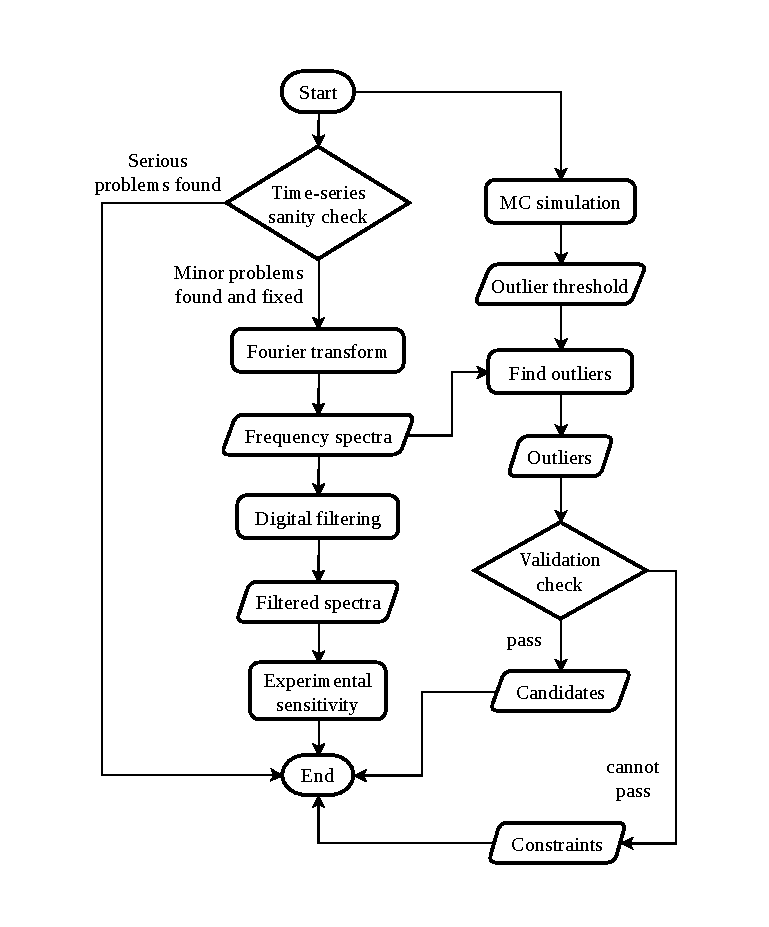
\includegraphics[width=0.99\linewidth]{figures/CASPEr-G-data-analysis-pipeline.drawio.pdf}
    \caption{Data-analysis pipeline for the CASPEr-Gradient search. Details of this pipeline are discussed in Section~\ref{sec:results:data_analysis:procedure}.}
    \label{fig:casper_g_data_analysis_pipeline}
\end{figure}
% the figure is made with draw.io
% figure width 130 mm
% font: Times New Roman, 15 px

\subsection{Procedure}\label{sec:results:data_analysis:procedure}

\subsubsection{Time-series sanity check}

Data with Gaussian noise are expected from the SQUID and LIA in the absence of an ALP signal.
In the presence of an ALP signal:
\begin{itemize}
    \item if the ALP signal is weak compared to the noise, the data are still approximately Gaussian;
    \item if the ALP signal is strong, the data are no longer Gaussian, and stochastic drift with a characteristic timescale set by the ALP coherence time is expected, as illustrated in Figure~\ref{fig:MW_axion_time_domain_stochastic}.
\end{itemize}
Moreover, when recording the data, instability and fluctuations in hardware and software could compromise data sanity.
Therefore, the first step in data processing is to check the sanity of the time series.
The time-series are checked for
\begin{enumerate}
    \item \textbf{Corrupted data values.} The data are first checked for \texttt{NaN} (not-a-number) or infinite values. Since the time-series are stored as \texttt{numpy} arrays, NaN and infinity are examined by \texttt{numpy.isfinite} and \texttt{numpy.isnan}.
    \item \textbf{Long-term instability (``drift'').} Slow (compared with the ALP coherence time) changes of the mean or variance due to unstable SQUID flux-locked-loop operation are tested within individual scan steps.
    \item \textbf{Short-term instability (``jumps'').} Local discontinuities or clusters of outlying samples in chunks much shorter than the ALP coherence time are searched for after the drift check. Such jumps may originate from magnetic noise due to mechanical or acoustic vibration, and can produce spectral leakage and artificial outliers in the search spectrum.
    \item \textbf{Non-Gaussianity.} Data without drift are tested for consistency with the Gaussian-noise assumption used in the threshold estimation.
\end{enumerate}
Depending on the problems found, the following approaches may be applied:
\begin{enumerate}
    \item \textbf{Time-series windowing.} If values in the data are found to be \texttt{NaN}, infinite values, jumps exceeding a certain threshold, or drifts, a window is applied to the time series to set the affected values to zero, so their effects are excluded.
    The window is designed to have a smooth envelope.
    The effects of the window on the average power of the data are later accounted for in the Fourier transform.
    \item \textbf{Baseline correction.} If the drift is attributed to unstable SQUID operation, the baseline is corrected by adjusting chunks of the time series to have a common mean. Otherwise, the affected data are excluded using a window with zero values. Uncorrected drift would produce low-frequency spectral structures.
    \item \textbf{Discarding.} If the fraction of invalid data exceeds a specified threshold, the corresponding measurement should be discarded. This threshold is arbitrarily chosen to be \SI{1}{\percent}.
\end{enumerate}

Note that features that do not match the ALP models investigated in this thesis, such as fluctuations on timescales much shorter than the ALP coherence time, may not be noise or faulty hardware/software behavior, but signals of other new physics.
It is wise to keep track of these features for future considerations.

% Data with unresolved drift would be reported.         for the discarded because it can create low-frequency spectral structure.

% Before constructing the frequency spectra, each recorded time series is tested for numerical validity and stability.
% The checks are applied to the organized time-series segments and determine whether a segment can be used directly, should be masked, or should be paused for manual inspection.

\subsubsection{Fourier transform and filtering}

Frequency spectra are generated by Fourier transforming time-series data that pass the sanity checks.
There are several forms of the frequency spectra, including the power spectrum (PS), power spectral density (PSD), and amplitude or linear spectral density (ASD or LSD).
These spectra are defined as
\begin{equation}
    \mathrm{PS} \propto \left|\mathrm{FT}[\mathrm{window(t)} \cdot s(t)]\right|^2,
\end{equation}
\begin{equation}
    \mathrm{PSD} = \frac{\mathrm{PS}}{\mathrm{ENBW}},
\end{equation}
and
\begin{equation}
    \mathrm{ASD} = \mathrm{LSD} = \sqrt{\mathrm{PSD}},
\end{equation}
where $\mathrm{FT}$ is the Fourier transform, $\mathrm{window(t)}$ is the window function, $s(t)$ is the time series, and $\mathrm{ENBW}$ is the effective noise bandwidth.
In the data analysis of CASPEr, $\mathrm{ENBW}$ is approximately the resolution bandwidth (RBW) \footnote{also known as spectral resolution or bin width} since the applied window function is approximately rectangular.
The exact formula of $\mathrm{ENBW}$ can be found in Equation (22) of Ref.\,\cite{Heinzel2002_SpectrumSpectralDensity}.
The power spectrum is normalized in a way that the sum of the spectra is the average ``power'' of the signal:\footnote{Usually, power is defined as the amount of energy transferred or converted per unit time. For a voltage signal in units of \unit{\volt}, the power is in the units of \unit{\volt^2\per\ohm}. However, the ``power'' in the spectral analysis is defined as the square of the signal; therefore the ``power'' of the signal has units of \unit{\volt^2}. This special but common definition is adopted in this thesis unless otherwise noted. }
\begin{equation}
    \mathrm{Average\,power} = \frac{\sum_{k=0}^{N-1}\left|\mathrm{window(t_k)} \cdot s(t_k)\right|^2}{\sum_{k=0}^{N-1}\left|\mathrm{window(t_k)}\right|^2}\,,
\end{equation}
where $N$ is the number of samples in the time-series, and $t_k$ is the time of the $k$-th sample.
When the window function is rectangular ($\mathrm{window(t)} = 1$ for all $t$), the average power is simply the sum of the power spectrum divided by the number of samples.
When the window function is not rectangular, the amplification or attenuation due to the window function is corrected by the sum of the window function squared in the denominator.
% Hence, the integral of $\mathrm{PSD}$ is also the average power, which explains why it is named as the density of power spectra.

After the frequency spectra are obtained, digital filters are applied for correction and SNR optimization.
Specifically, these steps consist of low-pass filter attenuation correction, baseline removal, and optimal filtering.

% First, the normalization of the frequency spectra is done under the convention that the
% after the time series are converted to a PSD with the DTRC attenuation and window corrections described in Ref.\,\cite{Heinzel2002_SpectrumSpectralDensity}, additional digital filters are applied to the spectrum for correction and SNR optimization.

% A window may be applied to the time-series ($\mathrm{window}\times\mathrm{time-series}$) to exclude insane data and avoid spectral leakage.

% There are many options how to implement digital low-pass filters. One common filter type is the
% exponential running average filter. Its characteristics are very close to those of an analog resistorcapacitor RC filter, which is why this filter is sometimes called a discrete-time RC filter. The
% exponential running average filter has the time constant as its only adjustable parameter. It
% operates on an input signal defined at discrete times , etc., spaced at
% the sampling time . Its output can be calculated using the following recursive formula,
% Second, the frequency-dependent attenuation due to low-pass filter is corrected.
The demodulated lock-in time-series experience digital low-pass filtering by the Zurich Instruments LIA\,\cite{ZurichInstruments_MFIA_UserManual}.
The output time-series can be calculated using the following recursive formula
\begin{equation}
    X_\mathrm{out}[k]=e^{-T_s/T_C} X_\mathrm{out}[k-1] + (1 - e^{-T_s/T_C}) X_\mathrm{in}[k] \,,
    \label{eq:XoutXinTC}
\end{equation}
where $X_\mathrm{in}$ and $X_\mathrm{out}$ are the input and output time-series arrays, $k$ is the sample index, $T_s$ is the sampling time, and $T_C$ is the time constant configured by the user.
% The recurrence requires an initial filter state.
For the first stored sample, $X_\mathrm{out}[-1]$ is chosen to be $X_\mathrm{in}[0]$ by convention.
This exponential moving average is also described as a digital discrete-time resistor-capacitor (DTRC) filter as it resembles the low-pass response of analog resistor-capacitor (RC) filters.
The time constant $T_C$ determines the \SI{3}{\decibel} bandwidth in the frequency domain.
Equation~\eqref{eq:XoutXinTC} describes a first-order DTRC filter.
Higher-order filters are implemented by cascading several filters in practice to suppress signals of frequencies much larger than the Larmor frequency ($|\mathrm{frequency}-\mathrm{Larmor\, frequency}|\gg\mathrm{NMR\, linewidth}$).
The response of the $n$-th-order filter in the frequency domain is approximated by the formula
\begin{equation}
    H_n(\nu)=\frac{1}{(1+i2\pi\nu T_C)^n} \,,
    \label{eq:H_nu_attenuation}
\end{equation}
where $H_n(\nu)$ is the $n$-th-order attenuation at frequency $\nu$.
This attenuation is corrected by dividing the PSD by the square of the absolute value of the attenuation.
% TODO check if the attenuation is H^2 or H^4 for PSD
If the time-series is Gaussian noise, the frequency spectra should be white noise after the low-pass filter correction, and the distribution of the PSD should follow a $\chi^2$ distribution. Since there are two channels in the lock-in amplifier, the degrees of freedom of the distribution should be two, i.e., a $\chi^2_2$ distribution.

Since the frequency-dependent attenuation in Equation~\eqref{eq:H_nu_attenuation} is only an approximation, the baseline of the PSD is not absolutely flat after the DTRC filter correction.
The curve of the baseline is estimated by an SG filter and removed from the PSD.
In practice, the spectrum is divided into chunks of a bandwidth much larger than the expected ALP linewidth, and a first-order SG filter is applied to each chunk to estimate the baseline.\footnote{The first order is chosen so as not to affect the ALP signal. Higher-order SG filters can subtract part of the ALP signal from the spectrum.}
The estimated baseline is then subtracted from the spectrum, and the result is divided by the baseline to obtain the normalized power excess (NPE):
\[
  \mathrm{NPE}(\nu) = \frac{\mathrm{PSD}(\nu)}{\mathrm{Baseline}(\nu)} - 1\,.
  \label{eq:NPE_baseline}
\]

% The script calls \code{step.optimalFilter(filterStepX=OPTIMAL\_FILTER\_STEP\_X)}
% to convert the normalized excess spectrum into an axion-search statistic.
% The method supports two regimes. If the axion linewidth is smaller than the
% NoPulse RBW, the signal is treated as unresolved and each bin is converted
% directly to excess power. If the axion linewidth is resolved, the
% RBW-normalized AxionBloch template is used as the matched-filter kernel and is
% shifted across the search spectrum in steps of \code{filterStepX} axion
% linewidths.

% The method stores the filtered frequency grid, excess-power estimate,
% global and local noise estimates, filter stride, realized step size, and
% filtered normalized power excess \code{filteredNPE}. The example injects a few
% large artificial excursions into \code{filteredNPE} for debugging and then
% calls \code{plotOptimalFilterResult}, which plots the axion template, the mean
% of \code{onePulseSignal.PSD\_90deg}, raw PSD plus baseline, and filtered
% statistic.

The next step is to decide whether optimal filtering\footnote{also known as matched filtering} should be applied or not.
The optimal filter is a weighted average of neighboring frequency bins, with weights determined by the expected signal lineshape; this choice maximizes the SNR among linear filters for random noise.
If the ALP linewidth is broader than the RBW of the spectrum, the signal is resolved, which means the signal is spread over multiple frequency bins.
In this case, optimal filtering is applied to combine the signal power into a single bin.
Alternatively, if the ALP linewidth is narrower than the RBW, the signal is unresolved and optimal filtering is not applied.

% Spike removal: to be verified if this step is necessary
One of the procedures that was adopted in the previous CASPEr-Gradient analysis\,\cite{Walter2025_CASPErLFthermal} was the removal of narrow spikes in the frequency spectra.
The philosophy behind this procedure is that spikes with linewidths much narrower than the expected ALP linewidth could be radio-frequency interference (RFI), and are unlikely to be ALP signals, so they can be removed to avoid false positives and reduce noise.
However, this procedure is not applied in the analysis of the data presented in this thesis for three reasons. First, the stochastic nature of the ALP field can produce spiky ALP signals, as shown in Figure~\ref{fig:MW_axion_time_domain_stochastic}.
Moreover, RFI lines are expected to be stable in frequency and amplitude, and can be identified by repeated scans.
Lastly, the spikes are suppressed by optimal filtering and did not affect the outlier search in the real analysis.

After these filtering steps, the spectra are ready to be searched for outliers.

\subsubsection{Outlier threshold}\label{sec:results:data_analysis:procedure:outlier_threshold}

If the probability of a signal being a false positive is less than $\SI{2.87e-7}{}$, which is the probability of a Gaussian random variable exceeding five times its standard deviation $\sigma$, the signal is considered a $\SI{5}{\sigma}$ signal.
An illustration of the Gaussian distribution and the probability of a $\SI{5}{\sigma}$ signal is shown in Figure~\ref{fig:5sigma-Gaussian-chisq-distributions}\,(a).
Such signals are considered traces of new physics.
\begin{figure}
    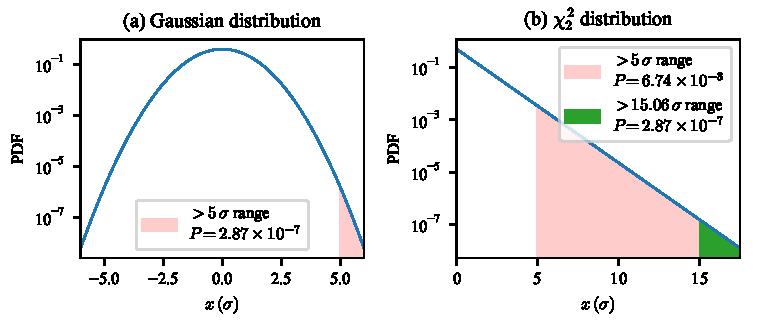
\includegraphics[width=0.99\linewidth]{figures/5sigma-Gaussian-chisq-distributions.pdf}
    \caption{The probability density functions (PDFs) of (a) Gaussian and (b) $\chi^2_2$ distributions.
    The probabilities of the shaded areas are noted in the legends. }
    \label{fig:5sigma-Gaussian-chisq-distributions}
\end{figure}

In addition to understanding what a $\SI{5}{\sigma}$ signal is, it is also important to understand what a $\SI{5}{\sigma}$ signal is not, and what is not a $\SI{5}{\sigma}$ signal:
\begin{itemize}
    \item Due to random noise, the measured amplitude of a $\SI{5}{\sigma}$ signal fluctuates rather than remaining $\SI{5}{\sigma}$ constantly\,\cite{Brubaker2017_HAYSTAC, aybas2021_SolidStateNMR}. If the noise is Gaussian, and if the noise is added to the signal linearly, the measured signal amplitude would be a Gaussian random variable with a mean of $\SI{5}{\sigma}$ and a standard deviation of $\sigma$, as illustrated in Figure~\ref{fig:5sigma-2-Gaussian_distributions}.
    \item A $\SI{5}{\sigma}$ signal is not always a signal that exceeds five times the standard deviation of the noise, unless the noise is Gaussian. For instance, if the noise follows a $\chi^2_2$ distribution, the threshold for a so-called $\SI{5}{\sigma}$ signal would be $\SI{15.06}{\sigma}$, as shown in Figure~\ref{fig:5sigma-Gaussian-chisq-distributions}\,(b).
    \item $\SI{5}{\sigma}$ signals are not rare, in terms of the number of events they represent. On one hand, $\SI{5}{\sigma}$ signals due to non-Gaussian noise are common in real experiments. On the other hand, experiments can accumulate huge amounts of data ($\gg 1/(\SI{2.87e-7}{})$ data points), and the probability of one $\SI{5}{\sigma}$ signal appearing due to random fluctuation is not negligible. This is also known as the look-elsewhere effect.
\end{itemize}

\begin{figure}
    \centering
    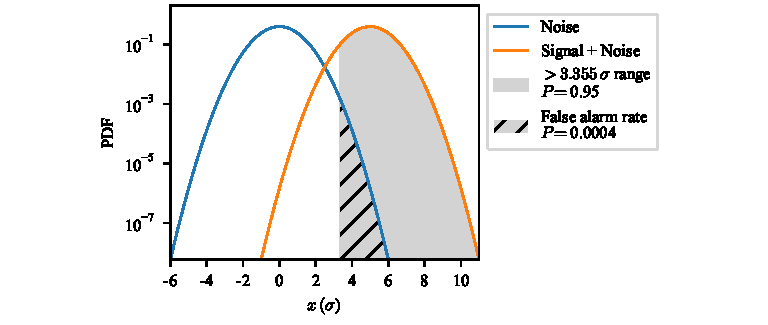
\includegraphics[width=1.0\linewidth]{figures/5sigma-2-Gaussian_distributions.pdf}
    \caption{Noise and signal amplitude distributions assuming Gaussian noise and linear signal dependence.}
    \label{fig:5sigma-2-Gaussian_distributions}
\end{figure}


The exotic $\SI{5}{\sigma}$ signals measured by CASPEr would appear as peaks in the NPE spectra.
To capture the $\SI{5}{\sigma}$ signals, a threshold is set, above which frequency bins are selected as outliers for further evaluation.

The value of the threshold should not be too low or too high.
If the threshold is too low, noise fluctuations are likely to be mistaken for signals (false positives).
If the threshold is too high, signals are likely to be missed (false negatives).
An appropriate threshold can either be determined by noise statistics or by MC simulations.
A common approach is to find a threshold that captures most signals while allowing a moderate number of noise fluctuations to pass.
In other words, this threshold corresponds to a certain confidence level (C.L.), such as \SI{95}{\percent}.
For example, if noise and signal are both Gaussian random variables with the same standard deviation $\sigma$ and different means (mean of noise being zero), a threshold of $\SI{3.355}{\sigma}$ is found to ensure that, in the presence of a $5\sigma$ signal, the chance of capturing the signal is \SI{95}{\percent}, and the chance of a false positive (false alarm rate) is only \SI{4e-4}{}, as illustrated in Figure~\ref{fig:5sigma-2-Gaussian_distributions}.
When the noise distribution is not Gaussian, the threshold can be determined by MC simulations, in which the noise and signal are simulated with the same statistics as in the experiment.

\subsubsection{NMR characterization}

The sample and the bias magnetic field are characterized by the following parameters and measurements:
\begin{enumerate}[label=\arabic*.]
    \item Larmor frequency, $T_2^*$, NMR linewidth and lineshape, polarization, and signal power measured by the free-decay signal after a \SI{90}{\degree} pulse.
    \item $T_2$ measured using a CPMG pulse sequence.
\end{enumerate}
These parameters are used to determine the sensitivity to ALP signals in the frequency band of interest.
Since these parameters may vary due to changes in the sample temperature, bias magnetic field, and other environmental factors, these measurements are performed at each scan step.

% For each scan step, the procedure is:
% \begin{enumerate}[label=\arabic*.]
%     \item \textbf{Calibrate the measurement.}
%     Fit the pulsed-NMR spectrum to determine the Larmor frequency, NMR linewidth, and signal power.
%     Together with the measured $T_2$, these quantities characterize the resonant response and convert SQUID output power into an equivalent transverse magnetization.

    % \item \textbf{Choose the signal statistic according to spectral resolution.}
    % Compare the predicted signal linewidth $\Delta\nu_{\mathrm{sig}}$ with $\delta\nu_{\mathrm{FFT}}$.
    % If the signal is resolved over several FFT bins, convolve the normalized PSD with the predicted ALP lineshape; this matched, or optimal, filter combines the signal power into a normalized power excess (NPE).
    % If $\Delta\nu_{\mathrm{sig}}\lesssim\delta\nu_{\mathrm{FFT}}$, the lineshape is not resolved and optimal filtering is not applied; the normalized excess power in the corresponding independent resolution element is used instead.
    % The MC calibration must reproduce whichever branch is used.

    % \item \textbf{Apply the detection threshold.}
    % Determine the rescan threshold from MC signal and noise realizations processed by the same pipeline.
    % Bins or resolution elements above the threshold are classified as outliers; those within $\pm5$ NMR linewidths of resonance are ALP candidates.

    % \item \textbf{Test candidates and set a limit.}
    % Merge candidates separated by less than one signal linewidth, compare them across repeated scans, and test whether they follow the expected resonant and modulation behavior.
    % If no candidate survives, convert the threshold power into a coupling limit after correcting for the simulated signal-recovery efficiency.
% \end{enumerate}

\subsubsection{Validation check and results}

Outliers that pass the threshold are not necessarily ALP signals.
Several methods are used to validate the outliers.
Those that can pass the validation tests are considered ALP signal candidates.

The key principle of the validation check is that ALP signals are expected to be consistent in terms of Compton frequency and coupling strength across measurements.
Following this principle, the outliers are examined by the following steps:
\begin{enumerate}[label=\arabic*.]
    \item \textbf{Merging outliers within individual scan steps by frequency.} The frequency of the outlier should be consistent within a certain tolerance. This tolerance is determined by the spectral RBW and the ALP linewidth. Outliers that appear at adjacent frequencies are likely to be the same ALP signal. Therefore, the first step in the validation check is to merge the outliers by their frequencies. The merged outlier is represented by the outlier with the largest amplitude.
    \item \textbf{Obtaining coupling strength.} The coupling strength of the ALP signal and its uncertainty can be obtained from the amplitude of the outlier, the NMR configuration, ALP periodic modulation, and the noise in the spectra.
    % \item \textbf{Finding interesting scan steps.}
    \item \textbf{Reproducibility.} The outlier should be reproducible across scan steps that cover the same frequency range. Though the coupling strength should be consistent, the amplitude of the outlier may vary due to the periodic modulation of the ALP signal and changes in the NMR configuration, especially the Larmor frequency. The outlier should be observed when and only when the estimated signal amplitude is significant compared to the noise level. This rule can be used to exclude outliers that are not reproducible across scans.
\end{enumerate}
In the absence of ALP candidates, the analysis sets constraints on the coupling strength as the minimum ALP coupling strength that can be observed at a given confidence level.
The constraint is determined by the NMR configuration and the ALP characteristics.
From the NMR characterization, the SQUID magnetic flux when the sample magnetization is tipped into the transverse plane, $\Phi_\perp(\nu)$, can be obtained from the PSD of the free-decay signal.
For a given ALP coupling strength $g_{\mathrm{aNN}}$, the tipping angle $\xi$ of the sample magnetization is determined by the Rabi frequency of the ALP field $\Omega_a \propto g_{\mathrm{aNN}}$ (given in Equations~\eqref{eq:Omega_a_MW} for Milky Way ALP and \eqref{eq:Omega_a_EH} for Earth-halo ALP) and the effective coherence time $T_\mathrm{coh}$ (given in Equation~\eqref{eq:T_coh}).
The PSD signal is therefore $\left(\xi\, \Phi_\perp(\nu)\right)^{1/2}$.
Under the assumption that ALP coupling is weak, the tipping angle is small and $\sin\xi \approx \xi$.
In the absence of an $n\,\sigma$ ALP signal at a certain confidence level,
\begin{equation}
    \left(\Omega_a T_\mathrm{coh} \, \Phi_\perp(\nu)\right)^{2} \leq n\,\sigma
    \,,\label{eq:gaNN_lim_equation}
\end{equation}
solving which gives the constraint on the ALP coupling strength $g_\mathrm{aNN}$ as a function of frequency.
% \begin{equation}
%     |g_\mathrm{ap}| \leq \sqrt{\frac{e_5}{\eta_\mathrm{rec}\,P_{\perp,1}}}
%     \,,\label{eq:limcouple-2}
% \end{equation}
% where $e_5$ is the signal power corresponding to the $\SI{5}{\sigma}$ NPE threshold, $P_{\perp,1}$ is the reference signal power for $|g_\mathrm{ap}|=\SI{1}{\GeV^{-1}}$, and $\eta_\mathrm{rec}$ is the analysis efficiency defined above.
If a candidate is observed, then the constraint at the candidate frequency is set by the coupling strength of the ALP candidate, below which a candidate was observed.

% section{Data-analysis details}\label{sec:results:analysis}

% This section gives the implementation details for the resolved standard-halo signal considered in the methanol search.
% Each \SI{100}{\s} time series is converted to a PSD and processed according to the procedure summarized in Section~\ref{sec:results:data_analysis}.

% subsection{Spike suppression}

% A narrow Savitzky-Golay (SG) filter with a window half-width equal to half the expected ALP linewidth at the scanned frequency is applied to the PSD.
% The residual between the raw PSD and the filter output is fitted with a $\chi^2_2$ distribution.
% Bins that deviate from the filter response by more than the fitted threshold, together with their four nearest neighbors, are replaced by the local filter average.
% This step suppresses narrow EMI spikes while preserving potential ALP signals.
% In the primary scan, only \SI{0.002}{\%} of bins were modified in this way.

% subsection{Baseline removal}

% A reduced chi-square test on the spike-corrected spectrum reveals a non-flat baseline.
% A second, broad SG filter with a window of 200 ALP linewidths is applied to estimate this baseline.
% The spike-corrected spectrum is then normalized by subtracting and dividing by this baseline, producing a spectrum with a flat expected noise floor.

% subsection{Matched filtering and NPE}

% For the \SI{100}{\s} methanol data, the expected standard-halo ALP linewidth is much larger than the \SI{0.01}{\Hz} FFT-bin width, so the signal lineshape is spectrally resolved.
% A matched filter using the expected ALP signal lineshape $\lambda_\perp(\nu,\nu_a)$---the normalized spectral lineshape of the ALP-field gradient component perpendicular to $\mathbf{B}_0$, as given in Ref.\,\cite{Gramolin2022Feb_SpectralSignatures}---is therefore convolved with the normalized PSD.
% The result, normalized by its standard deviation, is the normalized power excess (NPE).
% The matched-filter step size is half the ALP linewidth.
% This filtering step would be omitted for an unresolved signal with $\Delta\nu_{\mathrm{sig}}\lesssim\delta\nu_{\mathrm{FFT}}$.


\section{Milky Way ALP measurement}\label{sec:results:MWALP20221223}

One proof-of-principle measurement was performed on December 23, 2022. This measurement is ideal for a Milky Way ALP search because it scanned the same frequency range three times and the duration of each scan step was long enough to cover multiple ALP coherence times.

\subsection{Experiment}\label{sec:results:MWALP20221223:experiment}

% parameters of the scans and covered frequency / mass range
The search covered a frequency band of
\begin{equation}
    \SI{1.348570}{\MHz}\pm\SI{120}{\Hz}\,,\nonumber
\end{equation}
corresponding to proton Larmor frequencies driven by a bias magnetic field $|\mathbf{B}_0| \approx \SI{31.67}{\milli\tesla}$.
This maps to ALP masses in a range of
\begin{equation}
    \SI{5.577237}{\neV/c^2}\pm\SI{496}{\femto\eV/c^2}\,.\nonumber
\end{equation}
% $5.576741$--$5.577733\,\unit{\neV}/c^2$
Three sequential scans over the same range were performed.
In each scan, there were over 40 scan steps, and the frequency step size was \SI{6}{\Hz}, approximately half the NMR linewidth, so that the NMR resonant windows of adjacent steps overlap.
% The most sensitive scan was treated as the primary scan and the other two (scans A and B) as consistency checks.

% about each scan step
At each frequency step, the following actions were performed in order:
\begin{enumerate}[label=\arabic*.]
    \item Free-decay measurement (one $\pi/2$ excitation pulse followed by a free-decay signal) to determine the Larmor frequency, linewidth, and NMR signal power. A Lorentzian fit to the resulting PSD peak extracts these parameters. %  $\Delta\nu$ (and hence $T_2^* = 1/(\pi\Delta\nu)$)
    \item $T_2$ measurement using a CPMG pulse sequence.
    \item \SI{100}{\s} measurement without any pulses. %, recording the SQUID feedback voltage $V_\mathrm{f}$ at \SI{13.4}{\kHz} sampling rate.
    \item Frequency step: the Larmor frequency is increased by $\approx \SI{6}{\Hz}$ by ramping the Helmholtz coils.
\end{enumerate}
Delays to allow ring-down noise to decay or the magnetization to return close to its equilibrium are applied between steps.
The measurement procedure is illustrated in Figure~\ref{fig:MWALP-meas_procedure}.
% The PSDs were recorded after demodulation of $V_\mathrm{f}$ by the lock-in amplifier; its reference frequency was detuned by \SI{820}{\Hz} from the Larmor frequency so that the NMR signal appears at a non-zero difference frequency, making it easily distinguishable from noise.
% Example PSD spectra and NMR characterization plots are shown in Figure~\ref{fig:measurements}.
% An example of the PSD spectra and NMR characterization from one scan step is shown in Figure~\ref{fig:MW_ALP-ALP-1Pulse-NoPulse-NPE}.
The experimental parameters and the relevant NMR and ALP characteristics are summarized in Table~\ref{tab:MWALP-meas}.

\begin{figure}[htb]
    \centering
    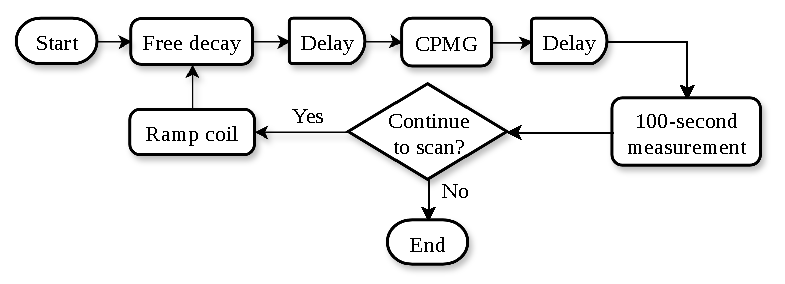
\includegraphics[width=0.99\linewidth]{figures/20221223_meas_diagram.drawio.pdf}
    \caption{Schematic of the Milky Way ALP measurement procedure.}
    \label{fig:MWALP-meas_procedure}
\end{figure}

% The measured relaxation times are $T_2^* = \SI{24.2\pm4}{\ms}$ and $T_2 = \SI{0.72(5)}{\s}$.
% Since $T_2^* \ll \tau_a \lesssim T_2$, the measurement falls in regime~(2) of Table~ref{}.
% The spectral factor is approximately $u \approx T_2^*/\tau_a \approx \SI{7}{\%}$.
% The ALP coherence time at the search frequency is $\tau_a \approx \SI{0.3}{\s}$, obtained from the ALP linewidth and Equation~\eqref{eq:taua_Qa_nua}.

\begin{table}[htb]
    \centering
    \caption{Technical parameters of the Milky Way ALP measurement on December 23, 2022 (Central European Time, UTC+1).  }
    \label{tab:MWALP-meas}
    \begin{tabular}{lc}
        \toprule
        Parameter & Name or value \\
        \hline
        Sample & thermally polarized methanol \\
        Number of scans & 3 \\
        Number of steps per scan & 45 \\
        Sweep coil current increment & \SI{0.8}{\mA} \\
        Frequency increment per step & \SI{6}{\Hz} \\
        Frequency scan range & $\SI{1.348570}{\MHz}\pm\SI{120}{\Hz}$ \\
        NMR linewidth in one step & $\SI{10}{\Hz}$ \\
        $T_2$ & $\SI{0.72(5)}{\s}$ \\
        ALP mass scan range & $\SI{5.577237}{\neV/c^2}\pm\SI{496}{\femto\eV/c^2}$ \\
        ALP linewidth $\Delta\nu_a$ & $\SI{1}{\Hz}$ \\
        ALP coherence time $\tau_a$ & $\SI{0.3}{\s}$ \\
        % SNR & $\approx 120$ \\
        Duration per step & $\SI{100}{\s}\, (\approx \SI{300}{\tau_a})$ \\
        Total duration & $\SI{6}{\hour} $ \\
        % spectral factor $u$ & $\approx \SI{10}{\percent}$ \\
        \bottomrule
    \end{tabular}
\end{table}

% \begin{figure}[htb]
%     \centering
%     
\includegraphics[width=.99\linewidth]{works/LF-thermal/figures/measurements.png}
%     \caption{\textbf{(a)} PSD after a $\pi/2$ pulse.
%     The NMR peak is fitted with a Lorentzian (red line); the center is at \SI{1.34844921(5)}{\MHz} with a FWHM of \SI{14.79(1)}{\Hz}.
%     \textbf{(b)} CPMG spin-echo amplitudes (blue dots) and exponential fit (red), giving $T_2 = \SI{0.72(5)}{\s}$.
%     \textbf{(c)} PSD of a \SI{100}{\s} ALP-search step.
%     The gray analysis window (\SI{8}{\kHz} wide) excludes filter artifacts near the band edges; the green resonant window ($\pm5$ NMR linewidths $=\pm\SI{70}{\Hz}$) is where ALP signal candidates are sought.
%     \textbf{(d)} Histogram of normalized power excess (NPE) derived from (c), with the rescan threshold $\Theta_\mathrm{RE}$ (red line) at the \SI{95}{\%} C.L. for a $\SI{5}{\sigma}$ ALP detection.
%     Reproduced from Ref.\,\cite{Walter2025_CASPErLFthermal} with permission.\YZ{a narrow frequency range for a and c? this figure may have to go to a different section}}
%     \label{fig:measurements}
% \end{figure}

% subsection{Expected ALP signal}

For the Milky Way ALP field, the expected linewidth near \SI{1.3}{\MHz} is approximately \SI{1}{\Hz}, corresponding to a coherence time of approximately \SI{0.3}{\s}.
Thus, each \SI{100}{\s} acquisition spans roughly 300 coherence times and measures the time-averaged stochastic signal power.

Over the 6-hour measurement, the ALP signal power varied between scan steps mainly because the Earth's rotation changes the component of the ALP-field gradient perpendicular to the bias magnetic field.
This predictable modulation, together with the measured NMR response at each step, is included when converting a power excess into an estimated coupling strength.
A plot of the effect of the Earth's motion on the expected ALP signal is shown in Figure~\ref{fig:ALP_wind_modulation}.
The annual modulation due to the Earth's motion in the solar system is included in the calculation, but it did not have a significant impact over the course of the measurement.
% Due to Earth's rotation, the component of the ALP-field gradient perpendicular to $\mathbf{B}_0$ varies over the course of the measurement.
% The resulting daily modulation of the signal amplitude is predictable and was tracked over the approximately 6-hour duration of the scans.

\begin{figure}[htb]
    \centering
    
\includegraphics[width=.6\linewidth]{works/LF-thermal/figures/ALP_wind_modulation.png}
    \caption{ALP parameters modulated by Earth's motion.
    Plotted for the start times of each measurement step for each of the three scans in seconds. Zero time corresponds to the start of data taking on December 23, 2022, 15:47:30 (Central European Time, UTC+1).
    Vertical dashed red lines mark the starts of each scan.
    Green line: $\sin\alpha$ oscillates with a period of one day.
    Blue dots with error bars: expected ALP signal powers in the PSD, according to Equations~\eqref{eq:squidpickup} and \eqref{eq:SQUID_beta}, for the reference case of an ALP gradient coupling to protons of $g_\mathrm{ap}=\SI{1e-9}{\GeV^{-1}}$.
    Uncertainties for these values were propagated from uncertainties in the spin relaxation times $T_2$ and $T_2^*$, sample Larmor frequency and NMR signal power. Reproduced from Ref.\,\cite{Walter2025_CASPErLFthermal} with permission. }
    \label{fig:ALP_wind_modulation}
\end{figure}

\subsection{Data analysis}
The technical details of the data analysis, following the procedure described in Section~\ref{sec:results:data_analysis:procedure}, are presented.
% subsubsection{Time-series sanity check}

% examples of jumps and how jumps are handled with masks. one figure

% subsubsection{Fourier transform and filtering}

After the time-series sanity checks, each \SI{100}{\s} record with windowing was Fourier transformed and corrected for the DTRC filter.
The spectral baseline was estimated with a first-order SG filter and removed to form the NPE spectrum.
For this search, $\mathrm{RBW} = 1/\SI{100}{\s} = \SI{0.01}{\Hz}$, whereas the expected ALP linewidth is approximately \SI{1}{\Hz}; the signal is therefore resolved over many frequency bins.
The optimal filter was applied to the NPE spectrum, using the expected ALP lineshape as the filter kernel.
One example of the spectra after different filtering steps is shown in Figure~\ref{fig:MW_ALP-ALP-1Pulse-NoPulse-NPE}.

% put a figure of the spectra after different filtering steps

\begin{figure}[htb]
    \centering
    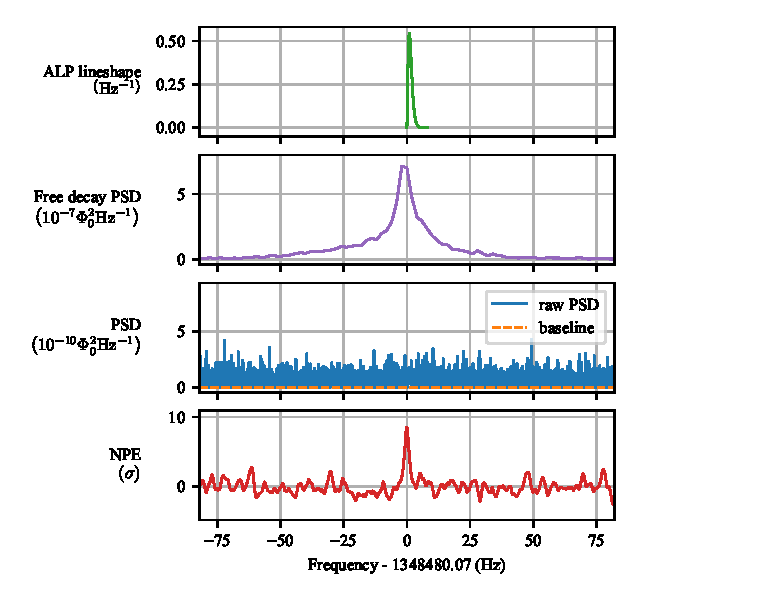
\includegraphics[width=.99\linewidth]{figures/MW_ALP-ALP-1Pulse-NoPulse-NPE.pdf}
    \caption{Example of data processing with an artificial ALP signal injected at the center of the spectrum. Top to bottom: lineshape of normalized ALP field, free-decay PSD, PSD of the measurement, and NPE. }
    \label{fig:MW_ALP-ALP-1Pulse-NoPulse-NPE}
    % script: CASPErG\examples\LF-science-runs\MW-axion-analysis-20221223\example_fig-MW_ALP-ALP-1Pulse-NoPulse-NPE.py
\end{figure}

% subsubsection{Outlier threshold}

MC simulations were performed to determine the threshold for recovering a $\SI{5}{\sigma}$ ALP signal with \SI{95}{\%} C.L.
Artificial $\SI{5}{\sigma}$ ALP signals were injected into simulated noise spectra before the optimal filtering, and the amplitudes of the filtered NPE were recorded.
Probability distributions of the filtered NPE were obtained from many realizations of the simulated noise and signal, and the outlier threshold $\Theta_\mathrm{RE}$ was determined from the distribution of the filtered NPE in the presence of a $\SI{5}{\sigma}$ ALP signal.
%
The simulations yielded $\Theta_\mathrm{RE} = 3.43$ with a false alarm rate of approximately $0.001$, as shown in Figure~\ref{fig:MC_simu-empirical_CDF}.

\begin{figure}[ht]
    \centering
    
\includegraphics[width=.6\linewidth]{works/LF-thermal/figures/Hypothesis.png}
    \caption{Empirical cumulative distribution function (CDF) obtained from the NPE distribution of spectra.
    The vertical dashed line represents the threshold for rescan, $\Theta_{\mathrm{RE}}$, corresponding to the null hypothesis of a $\SI{5}{\sigma}$ ALP detection at the \SI{95}{\%} C.L.
    The p-value corresponding to the threshold (horizontal dashed line) is approximately 0.001 (false alarm rate).
    Reproduced from Ref.\,\cite{Walter2025_CASPErLFthermal} with permission.
    }
    \label{fig:MC_simu-empirical_CDF}
\end{figure}


% subsubsection{Validation check}

% Frequency bins where the NPE exceeds the rescan threshold $\Theta_\mathrm{RE}$ are flagged as outliers.
% The threshold was determined via MC simulations of the NPE distribution under the null hypothesis that a $\SI{5}{\sigma}$ ALP signal is present, yielding $\Theta_\mathrm{RE} = 3.43$ at the \SI{95}{\%} C.L. (corresponding to a $p$-value of $0.001$).

% The overall analysis efficiency, accounting for the effect of baseline removal on signal recovery, was determined from simulations to be $\eta_\mathrm{rec} = \SI{88.2\pm4.6}{\%}$. This efficiency is applied when converting NPE values to coupling-constant limits.

\subsection{Results}\label{sec:results:MWALP20221223:results}

In order to include information about RFI and other non-white-noise structures, the data analysis searched for ALP signals in the frequency range of \SI{1.348570}{\MHz}\pm\SI{350}{\Hz}, much larger than the combined NMR linewidth of $\pm\SI{120}{\Hz}$.
This frequency range corresponds to \SI{700}{} Milky Way ALP linewidths at this frequency.
In the absence of an ALP signal, the number of outliers is expected to be \SI{.7}{} out of \SI{700}{} based on the false alarm rate (\SI{.1}{\percent}) obtained in the MC simulations.
In the analysis, \SI{58}{} outliers were found in the searched frequency range, which is much larger than the expected number of outliers due to non-white-noise structures that are not removed by the SG filters.
After the validation, \SI{6}{} candidates were identified among the outliers, listed in Appendix~\ref{app:candidates}.
No candidate appeared in the NMR resonant window.
Therefore, the search finds no statistically significant evidence for Milky Way ALP dark matter at the achieved sensitivity.

% Adjacent outliers within one ALP linewidth were first merged.
% By comparing the resonant window (within $\pm5$ NMR linewidths of the Larmor frequency) with off-resonance background, and by cross-checking across scans, these off-resonance outliers can be excluded.
% The on-resonance outliers were then compared across the three scans at consistent Compton frequencies.
% No candidate appeared in all three scans at consistent frequency within four ALP linewidths.
% The search therefore finds no statistically significant evidence for Milky Way ALP dark matter at the achieved sensitivity.
% Table~\ref{tab:candidates} summarizes the outlier counts and ALP signal candidates from all three scans.

% \begin{table}[htb]
%     \centering
%     \caption{Results of the three ALP scans.
%     $N_\mathrm{full}$: total NPE bins.
%     $X_\mathrm{full}$: outliers above rescan threshold.
%     $\langle X_\mathrm{full}\rangle$: expected value assuming white noise.
%     $N_\mathrm{res}$: bins in resonant windows.
%     $X_\mathrm{res}$: ALP signal candidates.
%     $\langle X_\mathrm{res}\rangle$: expected value.
%     $X'_\mathrm{res}$: candidates after merging those within one ALP linewidth.
%     $X''_\mathrm{res}$: candidates in this scan also appearing in the primary scan within four ALP linewidths.
%     Parenthetical fractions give the fraction of $N_\mathrm{full}$.}
%     \label{tab:candidates}
%     \begin{tabular}{lccc}
%         \hline\hline
%         & Primary scan & Scan A & Scan B \\
%         \hline
%         $N_\mathrm{full}$ & 481\,680 & 481\,680 & 481\,680 \\
%         $X_\mathrm{full}$ & 6393 (\SI{1.32}{\%}) & 5760 (\SI{1.20}{\%}) & 6202 (\SI{1.29}{\%}) \\
%         $\langle X_\mathrm{full}\rangle$ & 145 (\SI{0.03}{\%}) & 145 (\SI{0.03}{\%}) & 145 (\SI{0.03}{\%}) \\
%         \hline
%         $N_\mathrm{res}$ & 8430 & 8430 & 8430 \\
%         $X_\mathrm{res}$ & 5 & 7 & 3 \\
%         $\langle X_\mathrm{res}\rangle$ & 3 & 3 & 3 \\
%         $X'_\mathrm{res}$ & 5 & 5 & 3 \\
%         $X''_\mathrm{res}$ & --- & 0 & 0 \\
%         $\langle X''_\mathrm{res}\rangle$ & --- & 0 & 0 \\
%         \hline\hline
%     \end{tabular}
% \end{table}


% subsection{Exclusion limits}

In the absence of a detection, an upper limit on the ALP-proton gradient coupling is obtained from Equation~\eqref{eq:gaNN_lim_equation}.
In the NMR resonant bandwidth, the sensitivity is approximately $|g_\mathrm{ap}| \lesssim \SI{1e-2}{\GeV^{-1}}$.
The resulting exclusion limits are plotted in Figure~\ref{fig:ALPlimits}.

\begin{figure}[htb]
    \centering
    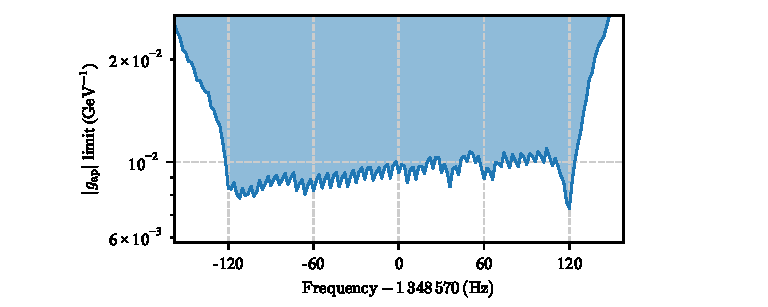
\includegraphics[width=\linewidth]{figures/MW_ALP-ALP_limits.pdf}
    \caption{ALP gradient-proton coupling excluded (indicated by the shaded region) at \SI{95}{\%} C.L. by the measurement on December 23, 2022. The sensitivity is good at \SI{1.348690}{\MHz} because the measurement duration was longer at this frequency. The sensitivity is worse at the edges of the scanned frequency range because the NMR response is weaker there. }
    \label{fig:ALPlimits}
\end{figure}

The measurement sets the limit $|g_\mathrm{ap}| \lesssim \SI{1e-2}{\GeV^{-1}}$ over the scanned ALP mass range $\SI{5.577237}{\neV/c^2}\pm\SI{496}{\femto\eV/c^2}$.
The sensitivity is limited by the polarization of the methanol sample; hyperpolarized samples are expected to improve it by multiple orders of magnitude.


\section{Earth-bound ALP measurement}\label{sec:results:EarthALP20221214}

% In this data taking, the bias magnetic field was ramped to ?? therefore the Larmor frequency of the sample was tuned to ??, corresponding to an ALP mass of \SI{}{\neV/c^2}.
% The measurement lasted for ?? hours in total. In this section, the measurement procedure and results are presented.

\subsection{Experiment}\label{sec:results:EarthALP20221214:overview}

One proof-of-principle measurement for the Earth-bound ALP halo model was performed on December 14, 2022 (Central European Time, UTC+1).
This measurement is suited to the Earth-bound search because each ALP-search acquisition per step lasted \SI{1}{\hour}, giving a narrow RBW for long-coherence-time signals.

The measurement scanned
\begin{equation}
    \SI{1.348575}{\MHz} \pm \SI{24}{\Hz} \nonumber
\end{equation}
by sweeping the magnitude of the bias magnetic field $|\mathbf{B}_0| \approx \SI{31.67403}{\milli\tesla}$.
This maps to ALP masses in a range of
\begin{equation}
    \SI{5.577258}{\neV/c^2} \pm \SI{99}{\femto\electronvolt/c^2}\,. \nonumber
\end{equation}
One scan over this range was performed.
There were 8 scan steps, and the frequency step size was \SI{6}{\Hz}, approximately half the NMR linewidth, so that the NMR resonant windows of adjacent steps overlap.

At each frequency step, the following actions were performed in order:
\begin{enumerate}[label=\arabic*.]
    \item Set the sweep coil current.
    \item Free-decay measurement (one $\pi/2$ pulse followed by a free-decay signal) to determine the Larmor frequency, linewidth $\Delta\nu$ (and hence $T_2^* = 1/(\pi\Delta\nu)$), and NMR signal power.
    A Lorentzian fit to the resulting PSD peak extracts these parameters and calibrates the sensitivity at each step.
    \item $T_2$ measurement using a CPMG pulse sequence.
    \item A 1-hour ALP measurement without any pulses.
    \item Free-decay measurement as in step 2.
    \item $T_2$ measurement as in step 3.
\end{enumerate}
Delays ($\gg T_1$) were inserted between pulsed-NMR measurements to allow the magnetization to return close to its equilibrium value along $\mathbf{B}_0$.
The measurement procedure is illustrated in Figure~\ref{fig:earthhalomeas_procedure}.
Note that the 1-hour ALP measurement duration is much longer than the 100-second duration used in the data taking described in Section~\ref{sec:results:MWALP20221223}.
The long measurement duration results in a much narrower RBW, which is beneficial for the sensitivity to ALP signals with long coherence time, such as the Earth-bound ALP halo.
% An example of the PSD spectra and NMR characterization from one scan step is shown in Figure~\ref{fig:EarthALP-measurements}.
The experimental parameters and the relevant NMR and ALP characteristics are summarized in Table~\ref{tab:earthmeas_params}.

\begin{figure}[htb]
    \centering
    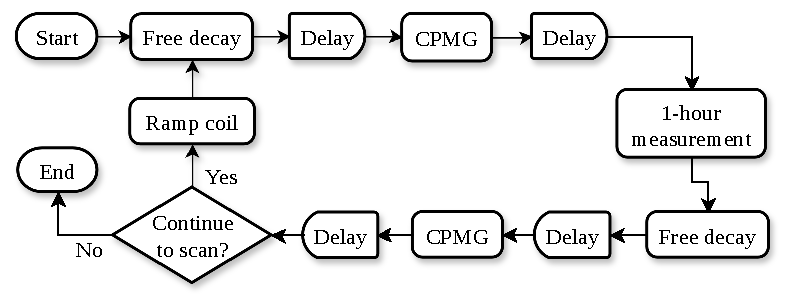
\includegraphics[width=0.99\linewidth]{figures/20221214_meas_diagram.drawio.pdf}
    \caption{Schematic of the Earth-bound ALP measurement procedure.}
    \label{fig:earthhalomeas_procedure}
\end{figure}

% \begin{figure}[htb]
%     \centering
%     \includegraphics[width=.99\linewidth]{figures/EarthALP-measurements.pdf}
%     \caption{Example PSD spectra and NMR characterization from one Earth-bound ALP scan step.
%     \label{fig:EarthALP-measurements}
% \end{figure}

\begin{table}[htb]
    \centering
    \caption{Technical parameters of the Earth-bound ALP measurement (December 14, 2022).}
    \label{tab:earthmeas_params}
    \begin{tabular}{lc}
        \toprule
        Parameter & Name or value \\
        \hline
        Sample & thermally polarized methanol \\
        Number of scans & 1 \\
        Number of scan steps & 8 \\
        Sweep coil current increment & \SI{0.8}{\mA} \\
        Frequency increment per step & \SI{6}{\Hz} \\
        Frequency scan range & $\SI{1.348575}{\MHz} \pm \SI{24}{\Hz}$ \\
        NMR linewidth in one step & $\approx\SI{10}{\Hz}$ \\
        ALP mass scan range & $\SI{5.577258}{\neV/c^2}\pm\SI{99}{\femto\eV/c^2}$ \\
        ALP linewidth $\Delta\nu_a$ & $\lesssim \SI{1}{\mHz}$ \\
        ALP coherence time $\tau_a$ & $\gtrsim \SI{1000}{\s}$ \\
        $T_2$ & $\approx\SI{2}{\s}$ \\
        % SNR (SNR) & $\approx 120$ \\
        Measurement duration per step & $\SI{1}{\hour}\,(\lesssim \tau_a) $ \\
        % spectral factor $u$ & $\lesssim 10^{-4}$ \\
        \bottomrule
    \end{tabular}
\end{table}


\subsection{ALP signal}


As mentioned in Section~\ref{sec:theory:earthALP:coherence}, empirical results are presented in this section under the assumption that the Earth-bound ALPs are mostly in the lowest-energy eigenstates, where the ALP density is significant at the Earth's surface.
For the 7 lowest-energy eigenstates of the Earth-bound ALP halo, the expected daily modulation\footnote{As discussed in Section~\ref{sec:theory:earthALP:periodic}, if no mechanism lifts the degeneracy, daily modulation would not be observed in the measurements. } of the ALP Rabi frequencies is shown in Figure~\ref{fig:EH_ALP-1s_to_5s-daily_modulation-Omega_a}.
Since CASPEr-Gradient is sensitive to the ALP-field gradient component perpendicular to the bias magnetic field, only the perpendicular component (polar and azimuthal) of the ALP Rabi frequency is relevant to the measurement.
A typical value of the Rabi frequency is approximately
\begin{equation}
    \Omega_{a,\,\perp}^{\oplus}
    \approx
    2 \pi \times \SI{.1}{\mHz}
    \frac{g_\mathrm{aNN}}{\SI{1e-9}{\GeV^{-1}}}
    \left(\frac{M_\mathrm{DM}^\mathrm{EH}}{\SI{4e-9}{M_\oplus}}\right)^{1/2}
    ~
    \label{eq:Omega_a_EH_perp}
\end{equation}
during the measurement.
This value is applied in the calculation of the ALP-proton gradient coupling in this section.
The tipping angle of the magnetization can be estimated as $\theta \approx \Omega_a T_2 \approx \SI{0.0002}{\pi}$.

\begin{figure}[htb]
    \centering
    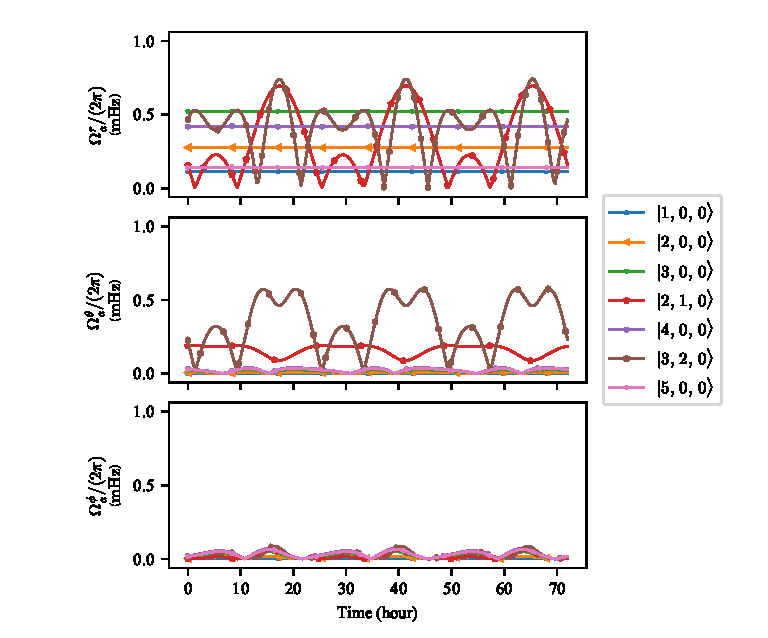
\includegraphics[width=\linewidth]{figures/EH_ALP-1s_to_5s-daily_modulation-Omega_a.pdf}
    \caption{Expected daily modulation of the ALP signal for the seven lowest-energy eigenstates ($m=0$) of the Earth-bound ALP halo, where the ALP density is significant at the Earth's surface. The ALP Compton frequency is taken as \SI{1.348500}{\MHz}. The Lorentz boost is included. The quantization axis is arbitrarily chosen to be along the Earth--Sun line. }
    \label{fig:EH_ALP-1s_to_5s-daily_modulation-Omega_a}
\end{figure}


% left as a free parameter, a few scenarios where measurements are sensitive to ALPs are considered here.
% Specifically, the 6 lowest-energy states of the Earth-bound ALP halo, where the ALP density is significant at Earth radius, are considered.
% Scenarios of ALP distributions are: ALPs distributed in individual eigenstates, or uniformly over the 6 lowest-energy eigenstates, as listed in Table~\ref{tab:EH_ALP-eigenstates}.
% The empirical results of these scenarios are presented in this section.

% \begin{table}[htb]
%     \centering
%     \caption{Frequency offsets and expected signal strengths for selected Earth-bound ALP eigenstates.
%     Scenarios of ALP distributed in individual eigenstates or uniformly over the 6 lowest-energy eigenstates are considered.
%     The frequency offset is calculated from the eigenenergy relative to the ALP rest energy, $\Delta\nu_a = E_\mathrm{eigen}/h- \nu_a$, where ALP Compton frequency $\nu_a$ is chosen to be $\SI{1.348575}{\MHz}$, the central frequency of the scan range.
%     The rms Rabi frequencies are calculated over the course of the measurement.
%     {The Rabi-frequency values are left open to be filled after the signal normalization is finalized.}}
%     \begin{tabular}{lcc}
%         \hline\hline
%         Eigenstate population & $\Delta\nu_a$ (\unit{\milli\hertz}) & rms $\Omega_a/(2\pi)$ (\unit{\milli\hertz}) \\
%         \hline
%         $1s$ & 0.198 & \YZ{TBD} \\
%         $2s$ & 0.539 & \YZ{TBD} \\
%         $3s$ & 0.757 & \YZ{TBD} \\
%         $2p$ & 0.788 & \YZ{TBD} \\
%         $4s$ & 0.895 & \YZ{TBD} \\
%         $5s$ & 1.005 & \YZ{TBD} \\
%         uniform over $1s$--$5s$ & - & \YZ{TBD} \\
%         % $3p$ & 1.021 & \YZ{TBD} \\
%         % $4p$ & 1.175 & \YZ{TBD} \\
%         % $5p$ & 1.247 & \YZ{TBD} \\
%         % $6p$ & 1.289 & \YZ{TBD} \\
%         \hline\hline
%     \end{tabular}
%     \label{tab:EH_ALP-eigenstates}
% \end{table}


% to be checked:
% n_r    l    Principal n    Name   Eigen E (eV)   Kinetic T (eV)  Mean v (m/s)
% -----------------------------------------------------------------------------
% 0      0    1              1s     8.194e-19       1.734e-20       8.680e+02
% 1      0    2              2s     2.228e-18       7.611e-19       5.751e+03
% 2      0    3              3s     3.130e-18       6.378e-19       5.265e+03
% 0      1    2              2p     3.258e-18       3.983e-19       4.160e+03
% 3      0    4              4s     3.702e-18       8.109e-19       5.937e+03
% 4      0    5              5s     4.158e-18       7.940e-19       5.875e+03
% 1      1    3              3p     4.222e-18       6.542e-19       5.332e+03
% 2      1    4              4p     4.860e-18       5.147e-19       4.730e+03
% 3      1    5              5p     5.158e-18       4.251e-19       4.299e+03
% 4      1    6              6p     5.329e-18       3.285e-19       3.779e+03

% For the scenarios of ALPs distributed in one single eigenstate, the expected ALP signal is a single frequency bin in the frequency spectra, in which case the optimal filter is not applicable.
% For the scenario of ALPs distributed uniformly over the 6 lowest-energy eigenstates, the expected ALP signal is expected to appear at the 6 discrete frequencies.
The differences between the eigenfrequencies of the Earth-bound ALP halo are on the order of \SI{1}{\milli\hertz}, while the difference between the $3s$ and $5s$ states is \SI{.25}{\milli\hertz}, as shown in Figure~\ref{fig:EH_ALP-state_amplitude-and-radial_wavefunctions-7states}.
For the \SI{1}{\hour} records used here, $\mathrm{RBW} = 1/\SI{1}{\hour} = \SI{.28}{\mHz}$, which is roughly the same order of magnitude as the ALP eigenfrequency differences.
Therefore, the signal is not well resolved in the frequency spectra, and the optimal filter is not applicable for this scenario either.


% In the reference frame where quantization axis is along the Sun-Earth direction, due to the daily rotation and the motion of the Earth, the component of the ALP-field gradient perpendicular to $\mathbf{B}_0$ varies over the course of the measurement.
% Using the ALP signal model established in Chapter~\ref{sec:theory:earthALP}, the expected Rabi frequencies of the pseudomagnetic field is calculated.
% In Figure~\ref{fig:EH_ALP-interference-daily-Omega_a}, the evolution of the expected Rabi frequency of the pseudomagnetic field is plotted.
% The rms Rabi frequencies are summarized in Table~\ref{tab:EH_ALP-eigenstates}.


% \begin{figure}[htb]
%     \centering
%     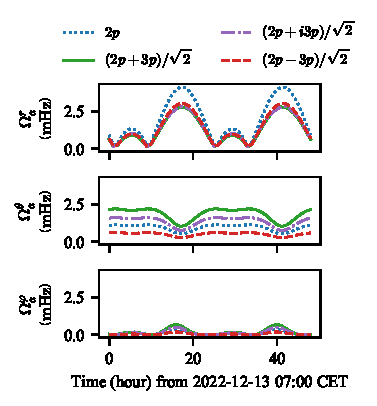
\includegraphics[width=0.6\linewidth]{figures/EarthHalo-interference-daily-Omega_a.pdf}
%     \caption{Expected evolution of the ALP-induced Rabi frequencies for the Earth-bound ALP halo model. Top to bottom: Rabi frequencies induced by gradients and Lorentz boost in radial, polar, and azimuthal directions. Scenarios of different state populations are considered as shown in the legend. The amplitude modulation is driven by the rotation of the laboratory frame relative to the ALP-field gradient.}
%     \label{fig:EH_ALP-interference-daily-Omega_a}
% \end{figure}


\subsection{Data analysis}
The technical details of the data analysis, following the procedure described in Section~\ref{sec:results:data_analysis:procedure}, are presented as follows.

% subsubsection{Time-series sanity check}

% Add examples of time-domain records, jumps, masks, and data-sanity cuts for the one-hour no-pulse acquisitions.
Short-term instabilities (``jumps'') in the time-series data were observed.
% No problem was found in the time-series sanity check except for jumps.
% One example of the jumps is shown in Figure~\ref{fig:EH_ALP-jumps-example}.
The jumps are unlikely to be statistical fluctuations, since the jumps appear in clusters rather than being randomly distributed in time.
One possible explanation is that the jumps are magnetic noise caused by transient mechanical vibrations.
Another possible explanation is that the jumps are exotic signals, such as ALP domain walls.
This thesis does not further investigate these possible transient signals of new physics.
% The analysis of these transient signals is included in the Chapter~\ref{chap:conclusion}.
% \begin{figure}[htb]
%     \centering
%     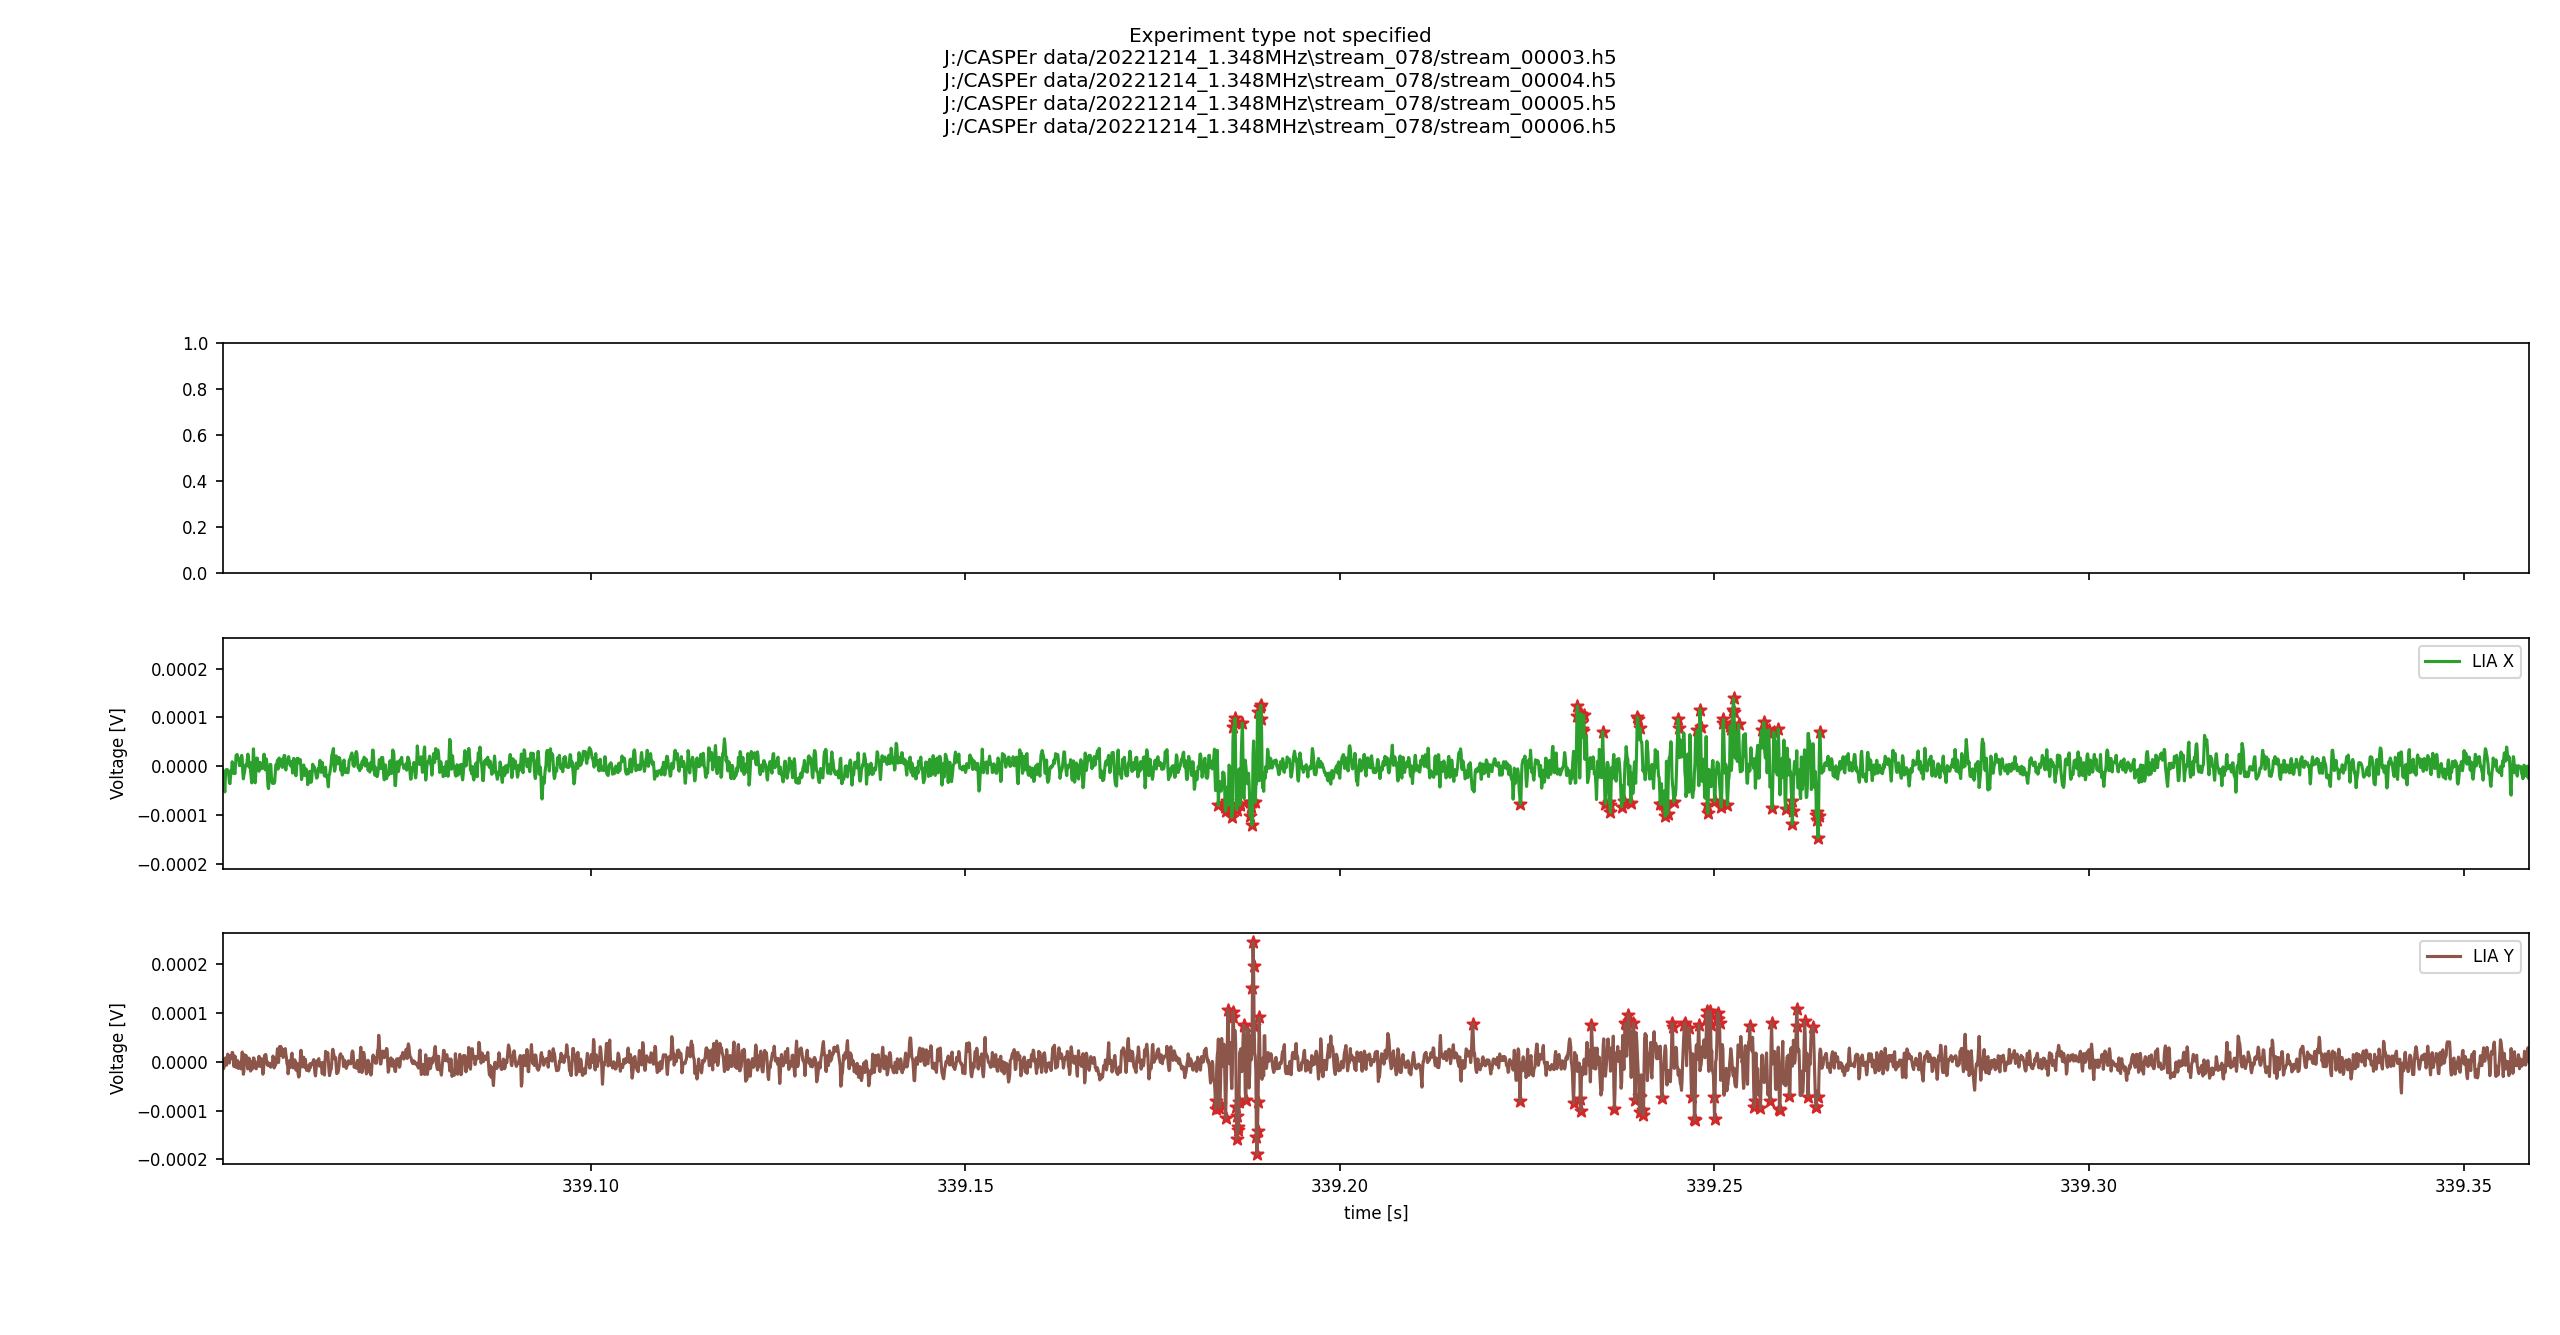
\includegraphics[width=0.99\linewidth]{figures/EH_ALP-jumps-example.png}
%     \caption{Example of jumps found in the time-series sanity check.\YZ{update this figure later.}}
%     \label{fig:EH_ALP-jumps-example}
% \end{figure}


% subsubsection{Fourier transform and filtering}
After the jumps were removed by applying windowing, Fourier transforms were performed to generate the frequency spectra.
The NPE spectrum was later formed after lock-in low-pass correction and the baseline subtraction.

% subsubsection{Outlier threshold}

% Determine the threshold for recovering a target Earth-bound ALP signal with the chosen statistic.
The time-series signals from the two LIA channels are independent and Gaussian, so the NPE follows a $\chi^2_2$ distribution.
As discussed in Section~\ref{sec:results:data_analysis:procedure:outlier_threshold}, a one-sided $\SI{5}{\sigma}$ outlier in Gaussian statistics corresponds to a $p$-value of $\SI{2.87e-7}{}$.
This $p$-value corresponds to $\SI{15.06}{\sigma}$ in the $\chi^2_2$ distribution.
In the presence of a $\SI{15.06}{\sigma}$ ALP signal, the NPE distribution is a non-central $\chi^2_2$ distribution.
If the outlier threshold is set at $\SI{7.809}{\sigma}$, the probability of capturing a $\SI{15.06}{\sigma}$ ALP signal is \SI{95}{\percent}, while the probability of a false positive (false alarm) is \SI{4e-4}{}.
Therefore, the outlier threshold is set at $\Theta = \SI{7.809}{\sigma}$ for the Earth-bound ALP search.
The threshold and corresponding probabilities are illustrated in Figure~\ref{fig:chisq-central-non_central-distributions}.
\begin{figure}
    \centering
    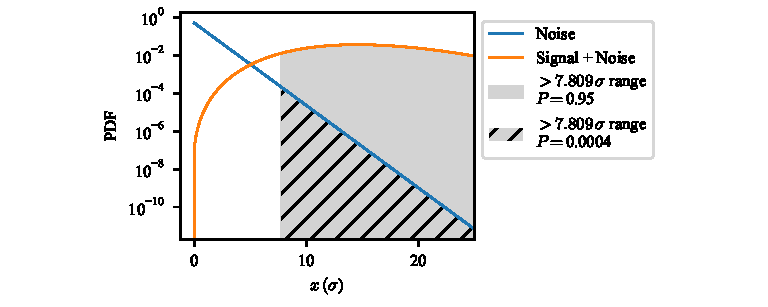
\includegraphics[width=\linewidth]{figures/chisq-central-non_central-distributions.pdf}
    \caption{Distribution of the NPE under the null hypothesis (white noise) and alternative hypothesis (ALP signal).}
    \label{fig:chisq-central-non_central-distributions}
\end{figure}


% \YZ{check if the frequency spectra is reversed}


% \begin{table}[htb]
%     \centering
%     \caption{Results of the Earth-bound ALP scan.
%     $N_\mathrm{full}$: total NPE bins.
%     $X_\mathrm{full}$: outliers above threshold.
%     $\langle X_\mathrm{full}\rangle$: expected value assuming white noise.
%     $N_\mathrm{res}$: bins in resonant windows.
%     $X_\mathrm{res}$: ALP signal candidates.
%     $\langle X_\mathrm{res}\rangle$: expected value.
%     \YZ{Adjust columns after the Earth-bound candidate definition is finalized.}}
%     \begin{tabular}{lc}
%         \hline\hline
%         & Earth-bound scan \\
%         \hline
%         $N_\mathrm{full}$ & \YZ{TBD} \\
%         $X_\mathrm{full}$ & \YZ{TBD} \\
%         $\langle X_\mathrm{full}\rangle$ & \YZ{TBD} \\
%         $N_\mathrm{res}$ & \YZ{TBD} \\
%         $X_\mathrm{res}$ & \YZ{TBD} \\
%         $\langle X_\mathrm{res}\rangle$ & \YZ{TBD} \\
%         \hline\hline
%     \end{tabular}
%     \label{tab:EarthALP-candidates}
% \end{table}


% \begin{figure}[htb]
%     \centering
%     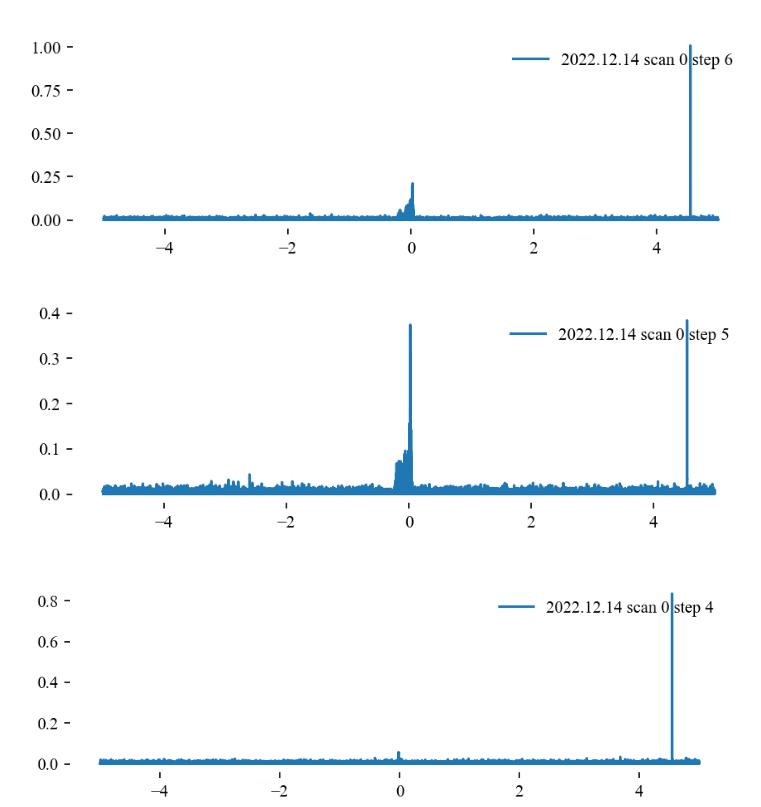
\includegraphics[width=\linewidth]{figures/EH_ALP-candidate-example.png}
%     \caption{Example of an Earth-bound ALP signal candidate.\YZ{modify the figure}}
%     \label{fig:EarthALP-candidate-example}
% \end{figure}

\subsection{Empirical results}\label{sec:results:EarthALP20221214:results}

% Frequency bins where the NPE exceeds the Earth-bound search threshold are flagged as outliers.
% Describe merging criteria, on/off-resonance windows, comparison between the pre- and post-search NMR calibrations, and treatment of single-scan candidates.

Since the expected Earth-bound ALP linewidth is narrower than the RBW, the ALP signal would not appear in more than two adjacent frequency bins.
The outliers were merged if they were adjacent.
After merging, 1041 outliers were found out of $\sim\SI{720000}{}$ NPE bins searched.
Based on the false alarm rate, the number of outliers is expected to be around \SI{288}{}.
The excess of outliers is likely due to non-white-noise structures such as RFI in the spectra.
There was no optimal filtering to suppress these structures.
% The corresponding coupling strengths of the merged outliers were obtained by the NMR characterization and Equation~\YZ{add equation ref here}.
Outliers appearing at consistent frequencies with consistent coupling strengths were considered candidates.
Out of the 1041 outliers, 38 candidates were found after the validation check.
% One candidate is shown in Figure~\ref{fig:EarthALP-candidate-example} as an example.
Note that only one scan was performed over the scan range, so the candidates cannot be cross-checked by multiple scans.
Most of the candidates did not appear in the NMR resonant windows; therefore, they are unlikely to be ALP signals.
Those candidates that appeared in the NMR resonant windows are likely to be aliases of RFI, since similar structures are observed in the spectra at regular intervals.
The candidates are listed in Appendix~\ref{app:candidates} for reference.

In the absence of a detection, constraints on the ALP-proton coupling can be derived from the measured NPE noise spectra and the expected signal power for the Earth-bound ALP halo model based on Equation~\eqref{eq:gaNN_lim_equation}.
At frequencies where candidates were found, the lower bounds of the constraints are set to the corresponding coupling strengths of the candidates.
In the NMR resonant bandwidth, the sensitivity is approximately $|g_\mathrm{ap}| \lesssim \SI{1e-9}{\GeV^{-1}}$.
The resulting exclusion limits are plotted in Figure~\ref{fig:EH_ALP-ALP_limits}.

\begin{figure}[htb]
    \centering
    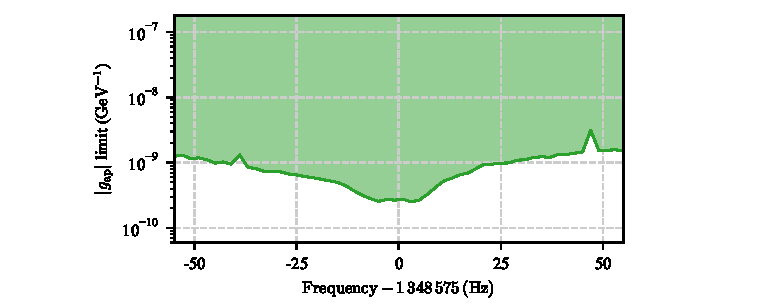
\includegraphics[width=\linewidth]{figures/EH_ALP-ALP_limits.pdf}
    \caption{ALP gradient-proton coupling excluded at \SI{95}{\%} C.L. by the measurement on December 14, 2022. }
    \label{fig:EH_ALP-ALP_limits}
\end{figure}
